\documentclass[12pt,a4paper]{article}
\usepackage[a4paper,margin=2.5cm]{geometry}

\usepackage[T1]{fontenc} 
\usepackage{mathptmx}
\usepackage{fontspec}\setmainfont{Times New Roman}
\usepackage{setspace}
\onehalfspacing
\usepackage{indentfirst}      % indent the FIRST paragraph too
\setlength{\parindent}{1cm}
\setlength{\parskip}{0pt}
\usepackage{amsmath,amssymb}
\usepackage{graphicx}
\usepackage{booktabs,array,multirow}
\usepackage{caption}
\usepackage{ragged2e}
\usepackage{tocloft}
\usepackage{titlesec}
\usepackage{hyperref}
 
\usepackage{microtype}
\usepackage{siunitx}
\usepackage{tikz}
\usepackage{pgfplots}
\pgfplotsset{compat=1.18}
\usetikzlibrary{arrows.meta,positioning,calc}
\usepackage{bbm}
\usepackage{csquotes}
\usepackage{float}
\usepackage{rotating}   % sidewaystable, for the wide robustness table
\usepackage{placeins}   % \FloatBarrier before the next section begins
\newcolumntype{L}[1]{>{\raggedright\arraybackslash}p{#1}}
 
\usepackage[style=apa,backend=biber]{biblatex}
\addbibresource{ref.bib}
 
\hypersetup{
    breaklinks,
    colorlinks,
    allcolors=black,
    urlcolor=blue,
}
 
%%==================================================================
\begin{document}
 
\begingroup\setstretch{1}\tableofcontents\endgroup
 
\thesischapter{Introduction}
\section{Introduction}\label{sec:intro}


\subsection{Overview}\label{subsec:overview}


\subsection{Hypothesis}\label{hypothesis}

The thesis hypothesis is as follows

\vspace{\baselineskip}

H1: Exchange rate volatility against Euro is significantly associated with real GDP in non-
Euro EU member states.
\vspace{\baselineskip}

H2: The relationship between exchange rate volatility and growth depends on euro-area
trade intensity, weakening as a country's trade with the euro area rises as a share of GDP.

\vspace{\baselineskip}

H3: The relationship between exchange rate volatility and growth is stronger in periods of
financial stress than in normal condition


 
\section{Theoretical Framework}\label{sec:theory}

\subsection{Theoretical Background}\label{theo_background}
    Six member states of the European Union have retained their own currencies instead of adopting the euro.
The theory of optimum currency area address whether adopting same currency carries a cost (\cite{mundell_theory_1961}).
Mundell posed the question of whether a group of countries should share the same currency and argued currency boundaries are
an economic question rather than political. 
Pointed out that the shared currency removes the transaction costs of conversion and eliminates the future exchange rate uncertainty.
The benefit of monetary both larger the intensity of trade between country and lower the cost of cross-border trade and investment.
While at the same time it showed the other side of adopting common currency, 
losing the two instruments where are the independency of monetary policy and the ability to adjust the nominal exchange rate.
When symmetric shock applied, members of common currency tend to react the same and the common policy response is broadly appropriate for all members since it impose a much smaller cost.
In the other hand, the asymmetric shocks impose a larger cost where the adjustment must occur through wages, prices and employments. 
It showed slower and costly effects because single policy can not suit countries needing opposite responses.

\vspace{\baselineskip}

Mundell (\citeyear{mundell_theory_1961}) proposed factor mobility as the criterion to judge whether the benefits outweigh the cost.
When labor can freely move between country migration from weaker demand to stronger demand would absorbs the asymmetric shock replace unemployment.
Hence, the exchange rate do not needed for adjustment.
When the cost of giving up the exchange rate is small in regions of high factor mobility and large in limited mobility.
Since there are no operating adjustment must occur through employment.
Mckinnon (\citeyear{mckinnon_optimum_1963}) argued the openness as an alternative criterion. 
When most of the consumption is imported in a very open economy, the prices are determined by partner's currency.
When the currency depreciates and rapid increase in import prices leading the domestic prices and wages rise in the same direction.
Therefore, the gain from the cheaper exports do not last.
The exchange rate become less useful to open economic than closed one. Giving up the their own currency cost less.
Another perspective showing diversification as third condition, arguing economy that's producing diversity of goods is less exposed to shocks, which reduce the need of the exchange rate to response (\cite{kenen_theory_1969}).

\vspace{\baselineskip}

Those conditions that mentioned above were intended to be checked before forming a currency union.
Frankel and Rose (\citeyear{frankel_endogeneity_1998}) argued that those are endogenous to the decision.
Adopting a common currency increase trade between countries which they tend to experience similar business cycle.
Therefore, the country failed the condition before might satisfy them after joining the currency union.
It showing the trades run in both directions which we should consider the reported result can be association rather than just a effect.
The condition we discussed only concern the decision of giving up a nation currency. 
And we will consider what a country can gain or loss by keeping their own currency.

\vspace{\baselineskip}

When demand of country's exports decrease, their goods become cheaper relative to trade partners. 
Friedman (\citeyear{milton_methodology_1953}) posed two scenarios can happen where the domestic wages and prices decrease, but the general wage levels resist.
The adjustment will be slow and happen through unemployment.
Alternatively, the currency can depreciate showing the same immediate change in relative prices.
Friedman argued it was easier to allow one price to move than adjust.   
With this argument the flexible exchange rate works as a main idea.

\vspace{\baselineskip}

We can take Friedman's argument as an implication for how exchange rate volatility should be interpreted.
When exchange rate acting as the adjustment function the volatility we can visibly observed in the function which can be explain just the adjustment work.
A currency moving according to a shock not necessarily a cost, it could be absorbing shocks.
We can consider volatility and macroeconomic instability are different where we cannot interpret the currency movement and economic performance without knowing what the currency is responding to.

\vspace{\baselineskip}

Against the argument we mentioned above that exchange rate movement can be treated as a cost.
Exchange rate volatility might discourage trade through uncertainty.
We consider a firm that agree a price in foreign currency and paid months later.
The domestic currency value of the payment is uncertain.
When the firm is not a risk taker will take certain payment over uncertain payment with same expected size.
The uncertain part of the payment make the transaction less attractive and trades that would be profitable will lost the gain they generated.
Even a firm with hedging strategy enter the forward contract with fixed exchange rate would not remove the problem.
There will be a cost in the contract and limited market for smaller currency contracts.
Consider a Polish's firm exporting to the euro area pays higher price for protection and gain less than a local firm operating in major currency.
The evidence that volatility actually reduce trade is weaker than the theoretical argument.
Clark et al. (\citeyear{clark_new_2004}) examined trade among 178 countries and find no robust evidence that exchange rate volatility has large negative effect on trade.
The volatility is not the major policy concern.
This does not mean the mechanism could not hold. 
It is difficult to measure uncertainty so the real effect may hard to detect.
This matter more to the countries that trade heavily with one partner instead size of the cost.
When a country's trade conducted with euro area larger share of the economy affected by the uncertainty of exchange rate.

\vspace{\baselineskip}

The two mechanisms we mentioned above point in opposite directions.
Exchange rate flexibility absorbs a shock supporting growth and at the same time exchange rate volatility increase the cost of trade.
Both mechanisms operate in floating currency where it can be observed as their net effect.
The theory suggests the balance between them depends on how exposed a country is to currency.
McKinnon's condition implies when there's more intensively an economy's trades with euro area the less value an independent exchange rate has.
Other argument implies an economy exposed to larger exchange rate uncertainty when they traded more with euro area.
Two arguments show the same conclusion where trade with euro area increase lead a flexible currency less useful and costly.
The theory predicts the effect of exchange rate volatility on growth is not constant.
But it decreases when country's trade with euro area increases.
It does not predict the effect of any level of trade integration and where two mechanisms offset another.
A further point from adjustment mechanism.
Flexible exchange rate absorbs shocks only when there are shocks can be absorb.
Therefore, in calm periods the relationship of mechanism is unlikely to be detectable in the data.
We will discuss both questions in the empirical part of the paper.


\subsection{Literature Review}\label{subsec:lit_review} 

The relationship between exchange rate volatility and economic growth has remained unsettled for decades with theory and evidence pointing in different directions (\cite{morina_effect_2020}).
Theory shows negative effect on volatility by increasing cost of international transaction.
However, the estimated effects have varied with countries and different periods with the measure of volatility (\cite{clark_new_2004}).
Our focus here is the effect of volatility on growth and trade with behavior of the non-euro EU country.

\vspace{\baselineskip}

The study by Morina et al. (\citeyear{morina_effect_2020}) examines fourteen Central and Eastern European Countries over 2002 to 2018.
In this study volatility is measured from real effective exchange rate as a standard deviation and z-score, enters a panel growth regression.
They estimate the model with country fixed effects having rejected random effects on basis of Hausman test.
The control variables are government expenditure, gross fixed capital, inflation, trade openness and domestic credit to private sector.
Their analysis conducts in two stages, estimates the direct effect of the volatility on growth and interacting volatility with real interest rate, inflation and trade openness.
They found a significant negative effect of volatility on growth and positive effect of trade openness.
The interaction of real interest rate and inflation are found to reduce the negative effect of volatility.
Interaction between volatility and trade openness shows negative and insignificant at the ten percentage.
This trade interaction which is most relevant to the study is the least conclusive in result.
The measurement of volatility matters for the results.
Morina et al. (\citeyear{morina_effect_2020}) measures their volatility as average across a whole period. 
The calm and volatile periods are treated the same. 
It computed against a group of trading partners instead of a single currency.

\vspace{\baselineskip}

Other studies showed mixed evidences. Janus and Riera-Crichton (\citeyear{thorsten_pdf_2015}) show that a growth decrease might destabilize the exchange rate when foreign capital exits the economy.
They address real effective exchange rate with volatility of commodity terms of trade.
Estimate the model on an annual panel of OECD countries from 1980 to 2011.
It shows negative volatility with growth and one standard deviation fall in volatility associated with around two percentage points of additional growth.
They reports an important finding here. The Great Recession increased exchange rate volatility in the non-euro countries by 38 to 189 percent of the sample mean.
They used Denmark and Sweden as non-euro sample. This suggests exchange rate differ inside and outside euro area mainly during financial stress periods.

\vspace{\baselineskip}

There are several studies focus on how the currency move against the euro.
They indicate a measurement convention where object of study is exposure to a certain currency.
It measures exchange rates against that currency instead of a trade-weighted average.
Orlowski (\citeyear{orlowski_co-movements_2016}) studies co-movement between non-euro EU currencies and euro from 2000 to 2015.
Orlowski finds high co-movement for Hungarian forint, Czech koruna, Polish zloty, Swedish krona and Danish krone while Romanian leu showing little co-movement.
The co-movement rose during periods of financial crisis with Czech, Polish and Hungarian currencies (\cite{chomicz-grabowska_financial_2020})
Kobor and Szekely (\citeyear{kobor_foreign_2004}) find volatility in these countries against the euro is subject to regime switching.
It shows cross-correlations higher when both currencies are in the high volatility regime.

\vspace{\baselineskip}

Studies of volatility and growth tend to measure volatility by summary statistic computed by annual data.
While condition volatility models have been applied in studies of exchange rate movement rather than macroeconomic factors.
Bollerslev (\citeyear{bollerslev_generalized_1986}) generalized Engle (\citeyear{engle_autoregressive_1982}) study and introduced GARCH model which conditional variance of a series depends on recent financial shocks and variance.
This model was developed to response the features of financial data that fixed window standard deviation cannot represent.
For example periods of high volatility can follow even higher volatility.
So this model can estimate volatility for every observation in series instead of single period.
Latief and Lefen (\citeyear{latief_effect_2018}) estimate GARCH (1,1) and threshold GARCH (1,1) models with an AR(1) mean equation on daily exchange rate returns for seven South Asian countries over 1995 to 2016.
They use the result volatility series in panel regressions on international trade and foreign direct investment.
The volatility is positive with trade in Bhutan, the Maldives and Nepal and negative in Pakistan.

\vspace{\baselineskip}

Both theoretical and empirical literatures could not establish a clear relationship between exchange rate volatility and economic growth.
Theory shows two mechanisms working in opposite directions.
Empirical results show in many different way.
The evidence is least on the trade interaction which is the mechanism the theory relies on.
This paper examines the question for a group of countries that retained their currency in certain period.
Two research questions follow:

\textbf{Does exchange rate volatility against euro influence economic growth in the six non-euro European member states?}

\textbf{Does the effect of volatility on growth depend on the extent of country's trade integration with euro area?}
\section{Commercial and Currency Integration}\label{sec:commercial}
In previous section we discussed the economic theory when a group of countries should share a currency.
Those conditions do not explain what exactly happened in the European Union where all six countries we study belong to the single market.
Labor and capital can move freely between each other country and the euro area.
Although most of the six countries we study look like suitable candidates for adoption.
They have not adopted the euro and the reason are legal and political more than economic.
We will discuss how each currency has been managed since 2005 and how they are different from each other.

\vspace{\baselineskip}

\begin{figure}[htbp]
\centering
\hyphenpenalty=10000 \exhyphenpenalty=10000
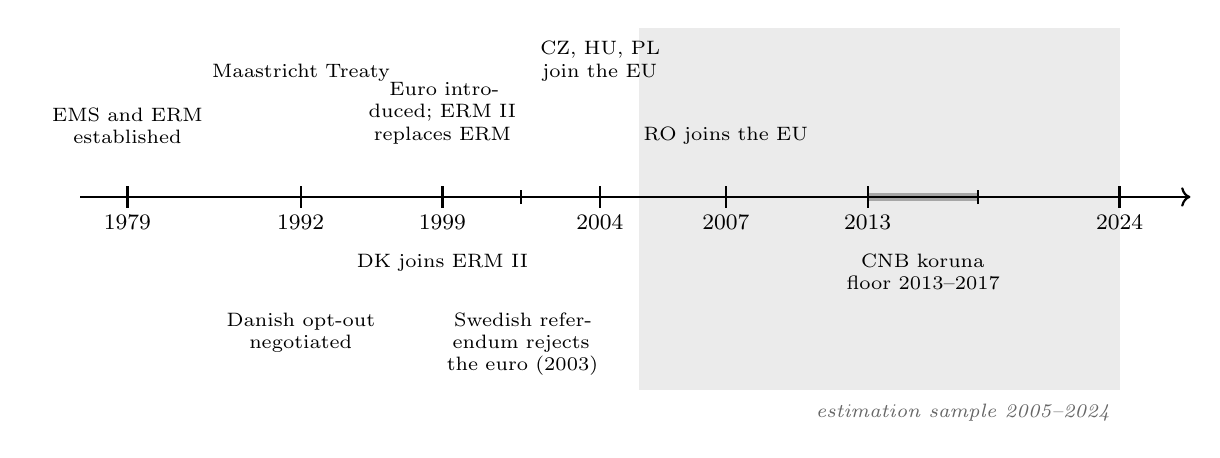
\begin{tikzpicture}[x=1.0cm, y=1cm]
% estimation window
\fill[black!8] (6.5,-2.45) rectangle (12.6,2.15);
\node[font=\scriptsize\itshape, black!60, anchor=north east] at (12.6,-2.5)
  {estimation sample 2005--2024};
% koruna floor span
\draw[line width=3pt, black!35] (9.4,0) -- (10.8,0);
% axis
\draw[->, thick] (-0.6,0) -- (13.5,0);
% ticks and years
\foreach \x/\lab in {0/1979, 2.2/1992, 4.0/1999, 6.0/2004, 7.6/2007, 9.4/2013, 12.6/2024}
  {\draw[thick] (\x,-0.14) -- (\x,0.14);
   \node[font=\footnotesize, below=3pt] at (\x,0) {\lab};}
\draw[thick] (5.0,-0.09) -- (5.0,0.09);
\draw[thick] (10.8,-0.09) -- (10.8,0.09);
% euro area institutions, above the line
\node[font=\scriptsize, align=center, anchor=south, text width=2.3cm] at (0,0.55)
  {EMS and ERM established};
\node[font=\scriptsize, align=center, anchor=south, text width=2.3cm] at (2.2,1.35)
  {Maastricht Treaty};
\node[font=\scriptsize, align=center, anchor=south, text width=2.5cm] at (4.0,0.55)
  {Euro introduced; ERM~II replaces ERM};
\node[font=\scriptsize, align=center, anchor=south, text width=2.3cm] at (6.0,1.35)
  {CZ, HU, PL join the EU};
\node[font=\scriptsize, align=center, anchor=south, text width=2.3cm] at (7.6,0.55)
  {RO joins the EU};
% national currency decisions, below the line
\node[font=\scriptsize, align=center, anchor=north, text width=2.3cm] at (2.2,-1.35)
  {Danish opt-out negotiated};
\node[font=\scriptsize, align=center, anchor=north, text width=2.3cm] at (4.0,-0.6)
  {DK joins ERM~II};
\node[font=\scriptsize, align=center, anchor=north, text width=2.5cm] at (5.0,-1.35)
  {Swedish referendum rejects the euro (2003)};
\node[font=\scriptsize, align=center, anchor=north, text width=2.6cm] at (10.1,-0.6)
  {CNB koruna floor 2013--2017};
% row labels

\end{tikzpicture}
\caption{Calendar of European monetary integration and the estimation window (2005--2024).}
\label{fig:timeline}
\end{figure}

Before turning to the main point, it is worth setting out the historical background and the conditions for joining the euro.
The monetary European Monetary was set up in 1979 to keep the exchange rate stable between members and encourage central banks working together (\cite{council_of_the_european_union_joining_2026}).
Currencies were kept within the agreed limits through Exchange Rate Mechanism.
Mutual agreement can change the rates which meant states gave up controls over their own currencies.
This system ended in 1999 when euro is introduced and the monetary policy passed to European Central Bank.
ERM II replaced the old mechanism which use as the framework for countries preparing to adopt the euro.

\vspace{\baselineskip}
\begin{table}[htbp]
\centering\small
\caption{Convergence criteria and the position of the six non-euro member states.}
\label{tab:convergence}
\begin{tabular}{L{2.4cm} L{4.2cm} c c c c c c}
\toprule
\multirow{2}{*}{\textbf{Criterion}} & \multirow{2}{*}{\textbf{Reference value}} & \multicolumn{6}{c}{\textbf{Fulfilled (2024)}} \\
\cmidrule(l){3-8}
 &  & CZ & DK & HU & PL & RO & SE \\
\midrule
Price stability & Inflation $\leq$ 1.5 pp above the three best performers & \emph{verify} & \emph{verify} & \emph{verify} & \emph{verify} & \emph{verify} & Yes \\
\addlinespace
Public finances & Deficit $<$ 3\% of GDP and debt $<$ 60\% of GDP & \emph{verify} & \emph{verify} & \emph{verify} & \emph{verify} & \emph{verify} & Yes \\
\addlinespace
Long-term interest rate & $\leq$ 2 pp above the three best performers & Yes & \emph{verify} & \emph{verify} & \emph{verify} & \emph{verify} & Yes \\
\addlinespace
Exchange rate stability & At least two years in ERM~II & No & Yes & No & No & No & No \\
\midrule
\multicolumn{2}{l}{Treaty obligation to adopt the euro} & Yes & No (opt-out) & Yes & Yes & Yes & Yes \\
\multicolumn{2}{l}{Public support for adoption (\%)} & 49 & \emph{verify} & \emph{verify} & 47 & \emph{verify} & \emph{verify} \\
\bottomrule
\end{tabular}
\caption*{\footnotesize Source: European Commission (2024) Convergence Report; Council of the European Union (2026).}
\end{table}
There are four conditions known as convergence criteria which a country must meet before adopt the euro.
It includes stable exchange rates where their inflation must be no more than 1.5 percentage points above the average of the top performing members.
The country needs stable public finances and sustainable interest rate. 
It government deficit must less than three percentage points of their GDP and its debt below 60 per cent.
And the long-term interest rates must be within two percentage points.
A country must spend at least two years in ERM II keeping its central rate close against the euro.
This condition matter more than others. This means a country can avoid adopting the euro by not joining ERM II.
And in this situation other three conditions do not matter.
Denmark is the exception case. It negotiated an opt-out from the treaties and do not required to adopt the euro.

\vspace{\baselineskip}

The six countries are outside of the euro area for different reasons. 
The Czech Republic, Hungry, Poland and Romania can be consider in one group.
None of four countries have joined ERM II.
The reason can be differ by countries and changed over time.
Most of them failed to meet the economic convergence criteria which including fiscal and inflation condition.
Out of the four countries only Czech Republic fulfilled the long-term interest rate criteria til 2024 (\cite{european_commission_european_2024}).
In the same report shows some countries lack of domestic political support.
Where Poland and Czech Republic are the lowest from six countries with 47 percentage and 49 percentage respectively.
Sweden fulfills all three condition except joining ERM II.
But the main reason it is the 2003 Referendum which Swedish public firmly voted against adopting euro with 56 percentage.
Denmark is the special case which they negotiated an exemption at Masstricht and they do not have obligation to adopt the euro.
They take part in ERM II and Danish krone close to fixed rate against the euro where central bank buy and sell to maintain it.

\vspace{\baselineskip}

The six countries managed their currencies in different ways and the differences are what make the comparison possible.
This was throughout the period we are studying from 2005 to 2024.
The Danish krone was closed to fixed rate against the euro for the whole period.
The krone barely move against the euro and it estimated volatility over the period is only a small fraction of the other countries.
The other five currencies floated but not in the same way.
The Czech National Bank operated currency floor regime against the euro from 2013 to 2017.
It prevented the koruna from strengthening beyond a stated level. 
This matter for the estimation.
The koruna was floating for part of the period and is held fixed til the end of the period.
It estimated persistence over the full sample sits close to the limit of what the model can do.
And the Romanian leu shows the same pattern for different reason.
Romanian leu is generally operating a managed float with central bank intervening more that its close countries.
The Sweden, Poland and Hungary currencies are floated and no comparable intervention.

\vspace{\baselineskip}

The six economics show differences in how much they trade with euro are same way as they manage their currencies.
Trade intensity means exports and imports measured as a share of GDP from the twenty euro area members.
Over the period it goes average from about 26 per cent in Denmark and 28 per cent in Sweden, to 37 per cent in Romania and 47 per cent in Poland, up to 85 per cent in Hungary and 88 in Czech Republic.
Czech Republic and Hungry are closely tied into German manufacturing where parts cross their borders many times before its sold.
Denmark and Sweden majorly trade with a wider set of partners where the United Kingdom and United States.
They have less of their trade in the euro.
Poland and Romania in between where they trade with euro area but their domestic economics are larger compare to the trades.

\vspace{\baselineskip}

The regime differences described above are not only the background.
It is worth to point out before the result are presented.
The exchange rate flexibility and trade exposure show different directions than the theory.
Denmark has the most fixed managed currency and the least euro are trade.
Opposite the Czech Republic and Hungry have freely floating currencies and the most euro trade.
McKinnon (\citeyear{mckinnon_optimum_1963}) shows the case more of a country trade with euro are the less its own currency is worth keeping.
The six countries show the opposite of what theory suggests which is why the interaction between volatility and trade is worth testing.

\vspace{\baselineskip}
All six of countries kept their own currencies for the whole study period.
Some studies grouped the countries by region often including the countries did adopt the euro and mixing the countries with and without their own exchange rate.
Morina et al. (\citeyear{morina_effect_2020}) report adoption was negative for growth over their period.
That is important because a sample containing countries with both sides cannot easily separate the effect of exchange rate volatility from the effect of joining the euro.
That is why the sample in this paper is on the same side.

\vspace{\baselineskip}

These currencies in sample except Danish krone are not permanently more volatile than the euro.
They are only volatile at certain periods.
Janus and Riera-Crichton (\citeyear{thorsten_pdf_2015}) find that the Great Recession raised volatility in the non-euro European countries by between 38 and 189 percentage of the sample mean.
The independent variable is the exchange rate volatility and regression can only find an effect where the variable moves.
When volatility is similar across these countries in calm periods and diverges during crises then the differences the model has to work with mostly from small number of years.
The relationship between volatility and growth should be easily show up in these years and hard to find in others.
We should consider it affects how weak result outside crisis periods meaning no relationship in calm periods.
This could also mean volatility are moving too little in the periods for a relationship to show up.
Two cannot easily be separated and we will discuss this later in the paper.

\section{METHODOLOGY}\label{sec:methodology}


\subsection{Data Collection}\label{subsec:data_col}

The model includes a wide range of macroeconomic indicators alongside the interactions.
Observations for all series run from 2005 to 2024 and the frequency is annual.
All series are sourced from the Eurostat database.
\begin{table}[H]
    \centering
    \caption{Macroeconomic series used in the model}
    \vspace{\baselineskip}
    \small
    \begin{tabular}{lll}
        \toprule
        Variable & Units & Eurostat ID \\
        \midrule
        Real GDP Growth($growth$) & Percentage & \href{https://doi.org/10.2908/NAMA_10_GDP}{NAMA10GDP} \\
        Euro-area Trade ($trade$) & Millions of Euro & \href{https://ec.europa.eu/eurostat/databrowser/bookmark/30053d9a-a5e9-42e8-abe6-5d9700efd145?lang=en&createdAt=2026-08-08T23:35:04Z}{DS045409} \\
        Government Expenditures($govexp$) & Millions of Euro & \href{https://doi.org/10.2908/GOV_10A_MAIN}{GOV10AMAIN} \\
        Investment($gfcf$) & Millions of Euro & \href{https://doi.org/10.2908/NAMA_10_GDP}{NAMA10GDP} \\
        Inflation ($hicp$) & Annual Average Rate of Change & \href{https://doi.org/10.2908/PRC_HICP_AIND}{PRCHICPAIND} \\
        \bottomrule
    \end{tabular}
    \vspace{\baselineskip}
    \caption*{\footnotesize Source: Eurostat. Note: Series are used in the model along with their Eurostat IDs.}
    \label{tab:eurostat_series}
\end{table}
The model consists of using the series defined in Table~\ref{tab:eurostat_series} to create variables and target as listed.

\begin{itemize}
    \item Target Variable: $growth_{t}$
    \item Variable of interest:
    \begin{description}
        \item[$X_{[t,\,1]}$] ($vol$)
        \item[$X_{[t,\,2]}$] ($trade$)
        \item[$X_{[t,\,3]}$] ($vol \times trade$)
    \end{description}
    \item Control Variable:
    \begin{description}
        \item[$X_{[t,\,4]}$] ($gfcf$)
        \item[$X_{[t,\,5]}$] ($hicp$)
        \item[$X_{[t,\,6]}$] ($govexp$)
    \end{description}
\end{itemize}
The sample includes Six European Union members that retained their own currencies.
The panel is annual from 2005 to 2024 giving 120 country year observations.
The reason that observations are taken from 2005 reflects three considerations.
The countries need to share the same institutional setting.
The Czech Republic, Hungary and Poland joined the European Union in May 2004 so 2005 is the first full calendar year in which they traded inside the single market alongside Denmark and Sweden.
Romania joined in 2007 two year after the start of the sample.
Its exchange rate against the euro and trade with the euro are are measured on the same basis.
Currency markets in Central and Eastern Europe were much thinner before joining the EU.
The early 2000s data reflect low trading volumes and more frequent central bank intervention than market behavior.
The twenty year sample window from 2005 cover multiple separated financial stresses.
Including the global financial crisis between 2008 to 2009, the euro area sovereign debt crisis between 2011 to 2012 and COVID-19 Shock from 2020.

\vspace{\baselineskip}

The dependent variable is real GDP growth taken as chain-linked volumes percentage change on the previous year.
A euro denominated series is not used.
It converts national GDP at the market exchange rate each year so a country whose currency weakens shows lower growth even it produced the same.
Since exchange rate volatility is the explanatory variable using it would build the relationship under test into dependent variable.

\vspace{\baselineskip}

Euro area trade intensity is the sum of import and export from twenty euro area members as a percentage of GDP.
There are no data for euro area aggregate for intra EU trade so the flows are taken from its international trades statistics and summed across the twenty partners.
The three controls are included gross fixed capital formation, general government expenditure and annual average rate of change of the consumer price.
Investment and government expenditure are expressed as shares of GDP using nominal GDP at current prices from the same source.
All variables are observed in percentage unit so their coefficients can be compared.
The exchange rate volatility is not observed directly as a published series. 
It is estimated from ECB daily euro reference rates where will be describe next.

\subsection{Exchange Rate Volatility Estimation}\label{subsec:vol_est}

Exchange rate volatility is estimated by a GARCH model and asymmetric threshold-GARCH model. The forms can be shown as GARCH(1,1) and TGARCH(1,1) with an AR(1) mean equation and $t$-student innovations.
It is following the specification in Latief and Lefen (\citeyear{latief_effect_2018})
The Daily log returns are computed as:

\begin{equation}\label{log_return}
r_t = \ln\left(\frac{S_t}{S_{t-1}}\right)
\end{equation}
    
where $S_t$ denotes units of national currency per euro. The mean and variance equations are

\begin{equation}\label{mean}
r_t = \beta_0 + \beta_1 r_{t-1} + u_t
\end{equation}

\begin{equation}\label{variance}
\sigma^2_t = \omega + \alpha u^2_{t-1} + \beta \sigma^2_{t-1}    
\end{equation}
where $\omega$ is constant, $\alpha$ and $\beta$ are coefficients. 
$\mu^2_{t-1}$ is the mean square of the previous time period.
$\sigma^2_{t-1}$ is the variance of the previous time period.
The Equation~\ref{mean} is the mean equation which represents the relationship between returns with its lag returns.
The Equation~\ref{variance} is the variance to explain the volatility.
\vspace{\baselineskip}

A normal distribution is not used for the errors.
Daily exchange rate returns contain more volatile movements than a normal distribution allows.
But the $t$-student distribution can allow this through its degrees of freedom parameter.
A threshold specification is estimated alongside the symmetric model.
It allows a depreciation and an appreciation of the same size to have different effects on the following day's volatility.


\begin{equation}\label{asymmetric}
\sigma^2_t = \omega + \alpha u^2_{t-1} + \gamma u^2_{t-1} d_{t-1} + \beta \sigma^2_{t-1}
\end{equation}

where $d_{t-1}=1$ when $u_{t-1}<0$ and $0$ otherwise.
Daily conditional volatility are aggregated to annual means to match the frequency of the macroeconomic data:

\begin{equation}\label{annual_vol}
VOL_{i,y} = \frac{1}{N_y}\sum_{t\in y}\sigma_{i,t}
\end{equation}

$N_y$ is the number of trading days in year $y$ for that currency.
The averaging method makes little difference to the result.
It matches the hypotheses which the average level of volatility a country faced during a year instead of how the volatility was distributed within it.
Averaging also explains why the results barely move between two volatility models.
Over around 250 trading days the differences between symmetric and threshold specifications cancels so the annual means are identical and follow the panel estimates.
This stability reflects the aggregation.

\subsection{Panel Regression Model}\label{subsec:reg_model}
The estimated volatility series enters a panel growth regression:
\begin{equation}\label{reg}
growth_{i,t} = \beta_0 + \beta_1\,vol_{i,t} + \beta_2\,trade_{i,t} + \beta_3\,(vol_{i,t} \times trade_{i,t}) + \gamma'X_{i,t} + \varepsilon_{i,t}
\end{equation}

\begin{equation}\label{reg_2}
growth_{i,t} = \beta_0 + \beta_1\,vol_{i,t} + \beta_2\,trade_{i,t} + \beta_3\,(vol_{i,t} \times trade_{i,t}) + \gamma'X_{i,t} + \mu_{i,t} + \lambda{i,t} + \varepsilon_{i,t}
\end{equation}

The Equation~\ref{reg} and Equation~\ref{reg_2} for country $i$ and time period $t$.
$growth$ is real GDP growth, $trade$ is Euro-area trade intensity, $X$ collects the three controls including $gfcf$, $hicp$ and $govexp$ as investment, inflation and government expenditure.
$\mu$ is the country fixed effects as dummy variable.
This gives each country its own baseline so the model compares a country with itself over time instead of the other five.
$\lambda$ is the year fixed effects as dummy variable.
Year fixed effects absorb what affects all six countries in the same year.
The year effects is important because these six countries trade mainly with the euro area and under the same shock periods.
The volatility rose and output fell in all of them at once in 2009 and 2020.
Without this year fixed effects cannot separate the two things apart.
It reads the crisis year collapse in growth as an effect of volatility.
The Czech Republic and 2005 are used as the baseline so $\mu_{CZ} = 0$ and $\lambda_{2005} = 0$.
Every other country and year effect is measured against them.
Which country and year are used makes no difference to the results.
Results are reported for pooled OLS, only country fixed effects and both country fixed effects and year fixed effects.

\subsubsection{Marginal Effects}\label{marg_ef2}

Because the model contains an interaction the coefficient on volatility does not describe the effect of volatility in general.
The effect of any other level of trade exposure is:

\begin{equation}\label{marg_ef}
\frac{\partial g}{\partial vol} = \beta_1 + \beta_3\, trade
\end{equation}

This is evaluated across the observed range of trade intensity and reported as marginal effects.
Reporting only the coefficient would describe one point on this range instead of the relationship.

\subsection{Estimation and Testing}\label{inf}

Standard errors show how each coefficient is estimated.
The usual formula assumes every observation carries independent information and that does not hold here.
The model is dependence within a country over time.
Growth in one year is related to growth next year and the estimated volatility is persistent so a country's errors are correlated to other years.
And its dependence across countries within a year.
All six countries trade mainly with the euro area and face the same shocks at the same time.
The volatility rose and output fell in together in 2009 and 2020 so the errors are correlated across countries.
Treating 120 observations as all independent evidence would overstate what the data can support and understate the true uncertainty around the estimates.

\vspace{\baselineskip}

Driscoll-Kraay standard errors are used because they allow for both forms of dependence.
Cluster by country handles correlation within a country but it works by treating each country as one independent.
So with six countries there are only six information which is too little for the method to give reliable standard errors.
Newey-West standard errors handle correlation over time but not across countries.
They also assume the data is one continuous series.
Because the panel is stacked by country.
Applying them means comparing Czech's last year with Denmark's first.

\vspace{\baselineskip}

Driscoll-Kraay standard errors make no assumption about how the errors are distributed.
The normality of residuals is not needed.
It is only for exact small sample tests and with 120 observation the result can be treated as large sample approximations.

\subsubsection{Coefficient Significance}\label{meth_coef}

Coefficients are tested for significance individually and jointly.
Individual significance is tested with $t$-tests which ask whether a single coefficient different from zero.
Individual tests are not enough because the model contains an interaction.
Volatility appears on its own and multiplied by trade intensity.
Testing them separately can also understate the relationship since the coefficients estimated together are not independent.
Three joint hypotheses are tested each using the Driscoll-Kraay covariance matrix:

\vspace{\baselineskip}

\begin{itemize}
    \item Trade intensity and the interaction are zero
    \item Volatility and the interaction are zero
    \item All three are zero
\end{itemize}
\vspace{\baselineskip}

Each tested with a Wald F-test.
Building the test on the Driscoll-Kraay covariance matrix means it carries the same robustness to serial correlation and cross country dependence as the standard errors
\subsection{Post-fit Validation}\label{post_fit}
The regression is checked after estimation to see whether the assumptions behind it hold.
Ordinary Least Squares produces estimates either way and gives no warning when assumption fail.
These tests work the other way from hypothesis tests.
Rejecting means something is wrong with the model and not rejecting means the assumption holds.

\begin{itemize}
    \vspace{\baselineskip}
    \item \textbf{Function Form:} Ramsey RESET. 
    This checks whether the relationship is really linear or whether something non-linear has left out.
    \vspace{\baselineskip}
    \item\textbf{Autocorrelation:} within country AR(1) on the residuals. 
    This checks whether one year's error predict the next.
    The residual is lagged within each country so no comparison crosses from one country to another.
    A pooled Durbin-Watson or Breusch-Godfrey statistic would compare Czech's last year with Denmark first year.
    \vspace{\baselineskip}
    \item\textbf{Heteroskedasticity:} Breusch-Pagan. 
    This checks whether the errors are equally spread across observation or larger for some than others.
    \vspace{\baselineskip}
    \item\textbf{Residual normality:} Jarque-Bera
    \vspace{\baselineskip}
    \item\textbf{Multicollinearity:} Variance Inflation Factor for all regressors.
\end{itemize}

\subsubsection{Variance Inflation Factors}

Variance inflation factors measure how closely each regressor moves with the others.
VIF is computed as:

\begin{equation}\label{meth_vif}
    \text{VIF}_j = \frac{1}{1- R_j^2}
\end{equation}

where $R_j^2$ comes from regressing $j$ on all the other regressors. 
The closer two regressors move together the harder it is to tell which one is producing an effect to one instead of the other and less precise both estimates become.

\vspace{\baselineskip}

The factors reported are for the estimated model in which volatility and trade intensity are centred in the Equation~\ref{reg} and \ref{reg_2}.
Volatility and trade intensity are centred by subtracting their sample means:

\begin{equation}\label{centring}
    \widetilde{vol}_{i,t} = vol_{i,t} - \overline{vol}, \qquad
    \widetilde{trade}_{i,t} = trade_{i,t} - \overline{trade}
\end{equation}

Centring does not change the fit.
The interaction coefficient, standard errors and residuals are identical either way but it changes what the individual coefficients mean.
Without centring the coefficient on volatility describes a country with no euro area trade at all.
It describes a country with average trade exposure when centred.

\vspace{\baselineskip}

When the interaction is formed before centring it shows higher factor.
Because trade intensity stays well above zero so the product is close to volatility scaled by a fixed amount.
The two move together.


\section{Results}\label{sec:results}
\subsection{Descriptive Statistics}\label{subsec:data_exam}

\begin{table}[H]
    \centering
    \begin{tabular}{lccccc}
        \toprule
        \textbf{Variable} & \textbf{N} & \textbf{Mean} & \textbf{SD} & \textbf{Min} & \textbf{Max} \\
        \midrule
        $growth$ & 120 & 2.40 & 3.07 & -6.70 & 9.30 \\
        $vol$ & 120 & 0.31 & 0.22 & 0.01 & 0.99 \\
        $trade$ & 120 & 51.60 & 26.19 & 23.56 & 100.82 \\
        $gfcf$ & 120 & 23.28 & 3.39 & 16.44 & 37.29 \\
        $hicp$ & 120 & 3.33 & 3.38 & -1.10 & 17.00 \\
        $govexp$ & 120 & 45.91 & 5.65 & 33.50 & 57.90 \\
        \bottomrule
    \end{tabular}
    \caption{Descriptive statistics for the estimation sample}
    \label{tab:descriptive}
\end{table}

The table \ref{tab:descriptive} presents the summary statistics for the estimation sample of 120 country and year observation.
The range of the exchange rate volatility which runs from 0.01 to 0.99 percentage measured as the annual mean of daily conditional standard deviations.
The lower end belongs to Denmark with its highest annual over the twenty year at 0.029.
It is still around ten times smaller than the average for any other currency in the sample.
This is the ERM II mechanism peg described before.
And the upper end belongs to the freely floating currencies in crisis years.

\vspace{\baselineskip}

The spread of trade intensity also stand out.
The standard deviation of 26.19 is half of its mean at 51.6 which is unusually large for macroeconomic variables.
This shows in the differences between countries instead of the movement over time.
The range from from 23.56 to 100.82 percentage of GDP runs from Denmark and Sweden at the lower end to Czech Republic and Hungry at the upper end.
It shows above one hundred percentage are not error. 
Trade counts the full value of goods crossing border which GDP counts only the value added at domestic so a country that import parts and re-export the assembled product count the same value twice in the trade.

\vspace{\baselineskip}

Growth ranges from -6.70 to 9.30 percentage with the negative end reflecting the recessions of 2009 and 2020.
Inflation ranges from -1.1 to 17 percentage covering both falling prices and the high inflation years of the late 2000s and 2020.


\begin{table}[H]
    \centering
    \begin{tabular}{lcc}
        \toprule
        \textbf{variable} & \textbf{centered} & \textbf{raw}\\
        \midrule
        $vol$                  &      1.25 &  5.91\\
        $trade$                &      1.19  & 4.75\\
        $vol x trade$          &      1.37  & 12.28\\
        $gfcf$                 &      1.25  & 1.25\\
        $hicp$                 &      1.34  & 1.34\\
        $govexp$               &      1.42  & 1.42\\
        \bottomrule
    \end{tabular}
    \caption{Variance inflation factors for the regressors.}
    \label{tab:vif}
\end{table}

Table \ref{tab:vif} presents variance inflation factors for estimated model and comparison for the same model with volatility and trade intensity on their original form.
In the estimated specification every factor ranges between 1.19 to 1.42 below the threshold of ten at which collinearity is usually a problem.
With the level below the threshold the regressors and coefficients can be read individually.

\vspace{\baselineskip}

The original form shows different result. Volatility, trade intensity and interaction rises to 5.91, 4.75 and 12.28 respectively.
The three controls remain unchanged since shifting a variable by a constant does not change its relationship to others.
Only the product is affected and with its two variables.
Nothing with the data is changed but only the point the variables are measured from.
Trade intensity multiplying volatility always means multiplying a large number.
The product is close to volatility scaled up by constants.
Two move together which is what VIF measures.
By centreing both variables on their own means and product no longer tracks volatility.
The high VIF number reflects where the variables are measured.
Since both versions produce identical coefficients, standard errors and residuals so the centred variables are the one matter.

\vspace{\baselineskip}

The correlations between variables do not exceeds 0.36 in absolute value (See Appendix~\ref{appendA} for further details).
The correlation between volatility and inflation is 0.29 so nominal exchange rate movement carries some inflation instability.
The correlation between volatility and growth is -0.08 close to zero which is what makes the conditional specification necessary.

\begin{figure}[H]
\label{fig:garchvol}
    \centering
    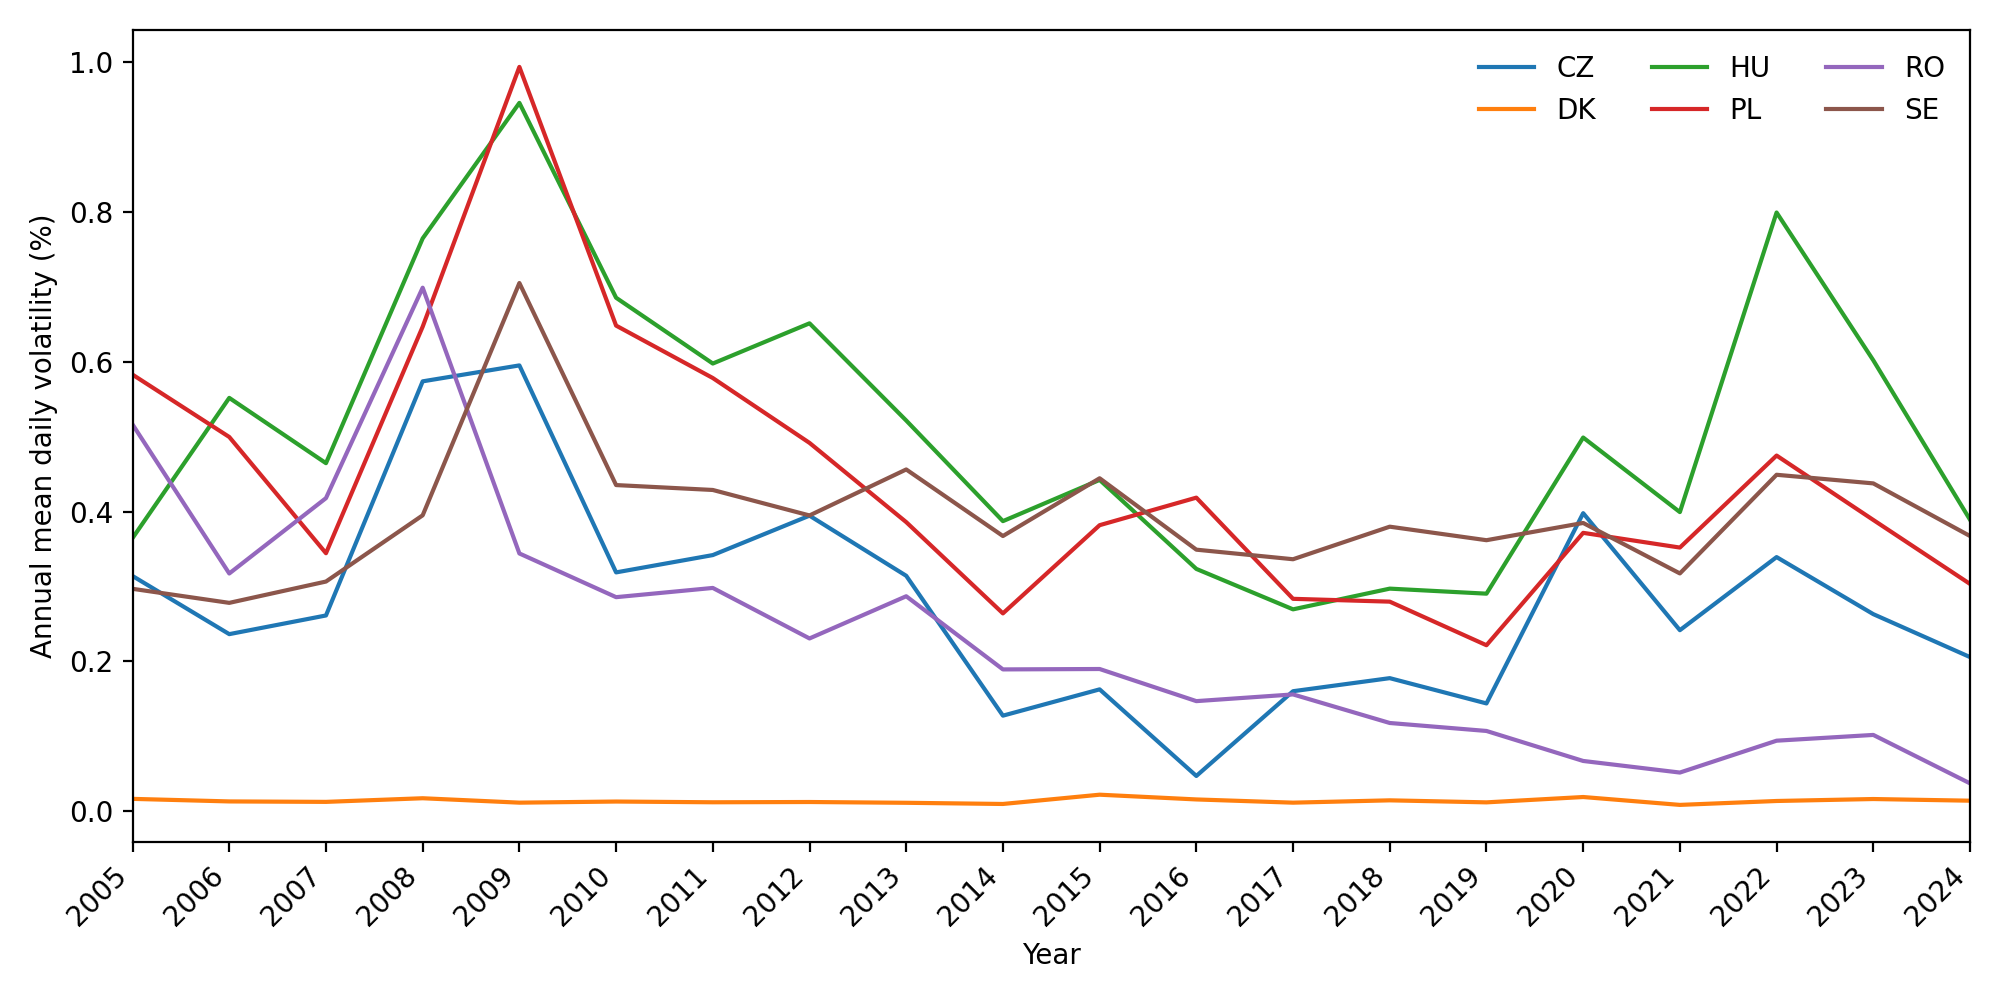
\includegraphics[width=0.75\textwidth]{fig/volatility.png}
    \caption{Annual Mean Conditional Volatility from GARCH(1,1)}
\end{figure}

Figure~\ref{fig:garchvol} presents the annual mean conditional volatility of each currency against the euro obtained from the GARCH(1,1).
As we expected the Danish Krone never rises above 0.03 in any year in the sample while other five currencies average between 0.26 to 0.52.
This the ERM II arrangement we discussed before.
The Danish Krone is held close to its central rate so there is very little movement for the model to measure.
GARCH describes how volatility changes over time and know Danish Krone barely moves.
The Danish Krone fit runs against the model's parameter limits.
This figure still measure how much the currency moved but the only record that the peg held instead of how volatility behaved.

\vspace{\baselineskip}

The clearest thing we can see from this figure is the fluctuation in 2009.
Volatility rises sharply in all five currencies peaking at 0.99 for the Polish zloty.
Both of the movement are more than double their sample averages.
This is exactly showing the global financial crisis and its the largest movement in the twenty years.
We can also see the other features from this figure.
The 2020 shock is much smaller than 2009 its volatility rises in that year but only to around 0.4 to 0.5.
And the second highest reading in the sample is not a crisis where the Hungarian forint reaches 0.8 in 2022 during European inflation.

\vspace{\baselineskip}

We can also spot different pattern in Czech koruna between 2013 to 2017.
It falls to 0.05 in 2016 the lowest recorded by any floating currency in the sample and recovers after 2017.
This is the Czech National Bank's exchange rate floor we mentioned and its effect on the estimation (See Appendix~\ref{appendB} for further details).
The koruna during this period is not a floating currency but interrupted as managed one.


\subsection{Regression Results}\label{subsec:panel}


\begin{table}[H]
    \centering
    \small
    \begin{tabular}{lccc}
        \toprule
        \textbf{Explanatory variable} & \textbf{Model 1} & \textbf{Model 2} & \textbf{Model 3} \\
        \midrule
        $vol$            & $-1.396$   & $-4.255$*** & $3.691$ \\
                              & $(1.443)$  & $(1.406)$         & $(2.331)$ \\[2pt]
       $trade$       & $0.000$    & $0.068$           & $0.051$* \\
                              & $(0.007)$  & $(0.082)$         & $(0.028)$ \\[2pt]
        $vol x trade$ & $-0.076$ & $-0.047$        & $-0.096$** \\
                              & $(0.061)$  & $(0.052)$         & $(0.048)$ \\[2pt]
        $gfcf$                  & $-0.007$   & $0.345$** & $0.263$*** \\
                              & $(0.098)$  & $(0.159)$         & $(0.085)$ \\[2pt]
        $hicp$                  & $-0.013$   & $-0.044$          & $-0.195$** \\
                              & $(0.090)$  & $(0.110)$         & $(0.092)$ \\[2pt]
        $govexp$ & $-0.169$*** & $-0.407$** & $0.019$ \\
                              & $(0.050)$  & $(0.194)$         & $(0.090)$ \\
        \midrule
        Country fixed effects & No  & Yes & Yes \\
        Year fixed effects    & No  & No  & Yes \\
        Observations          & 120 & 120 & 120 \\
        Number of countries   & 6   & 6   & 6 \\
        $R^2$                 & 0.151 & 0.347 & 0.787 \\
        Wald test & $F(6,113) = 3.337^{***}$ & $F(11,108) = 5.222^{***}$ & $F(30,89) = 10.962^{***}$ \\
        \bottomrule
    \end{tabular}
    \caption{Panel regression results. Driscoll--Kraay standard errors in
    parentheses. *** $p<0.01$, ** $p<0.05$, * $p<0.1$.}
    \label{tab:panel_results}
\end{table}

The table \ref{tab:panel_results} presents the regression under three specifications.
The first model pooled all 120 observations and treats them as one population.
The second model put in country as dummy variable.
The third model put in country and year together as dummy variables.
The standard errors are Driscoll-Kraay for this table.
We also computed the p-values under ordinary, Newey-West and cluster robust estimators (See Appendix \ref{appendC} for further details).
The estimates change very differently between specifications.
It is worth explaining the result since it determines which specification to use.

\vspace{\baselineskip}

The model 1 uses stacked panel of 120 country year rows and without fixed effects.
It shows nothing is significant except government expenditure.
The R-square shows 15 percentage which means only little variation in growth is explained by the model.
It is showing a poor fit and it is expected from this specification.
Because Denmark and Romania are very different economics and pooling them together means the model must explain the difference between a Danish year and a Romanian year using only six variables in the regression.
Most of the difference comes from things the model does not measure.

\vspace{\baselineskip}

The model 2 puts country fixed effect for stacked panel.
It is giving each country its own intercept as dummy variable and remove the problem.
This model no longer has to explain why Denmark grow differently from Romania on average.
It only has to explain why each country grows differently from its own average in given year.
The model fit improves to 35 percentage.
The volatility becomes significant with coefficient of -4.255.
It is saying that a country grows slowly in years when its currency is more volatile.
The country fixed effects model still cannot explain for what happened to all six countries in the same year.
The model 3 adding year effects with country effect changes the result.
Volatility loses its significance and coefficient changes to 3.691.
The interaction between volatility and trade intensity becomes negative at -0.096 and significant at the 5 percentage.
This model fits rises to 78.7 percentage.

\vspace{\baselineskip}

The coefficient on volatility changes sign between the two models which requires explanation.
The country fixed effects model compares each country with itself over time which removes everything fixed about the country itself.
Country effects cannot remove anything that hit all six countries in the same time which is the financial crisis.
In 2009 exchange rate volatility rose in every floating currency in the sample and output fell in every country.
The model observes high volatility and low growth and presents a negative relationship between them.
But the volatility and growth did not cause each other.
Both of them were consequences of the crisis and the model without the year fixed effect cannot tell the difference.

\vspace{\baselineskip}

Year effects solve this by giving each year its own intercept.
The 2009 crisis is now absorbed by the year effect so it can no longer show up in the volatility coefficient.
What it remains is the comparison whether a country whose currency was unusually volatile in a given year grew differently from one whose currency was not.
This comparison gives a different answer from the country fixed effects model and it is the one this thesis relies on.
So the model with both country fixed and year fixed specification is preferred for the rest of the analysis.

\vspace{\baselineskip}
The three control variables behave differently across the specifications and the pattern is informative.
Gross fixed capital formation is positive and significant under both fixed effects specifications at 0.345 and 0.263.
This is expected result where countries invest more in years when they grow more and two move together.
Inflation is significant only in the both fixed effects specification at -0.195.
Higher inflation goes with slower growth but only once year effects are included.
Before that inflation and growth were both moving with common cycle and the model could not separate the two.
Government expenditure shows in other way. 
It is significant in the first two models but not the third.
This suggests what looked like an effect was really the common cycle instead of specific to individual countries.
Adding year effects removes it.
A final point on how the volatility coefficient should be read.
The coefficient on volatility in the both fixed effects specification is not the effect of volatility in general.
Because volatility and trade intensity are centred.
It gives the effect for country with average euro area trade exposure.
It does not explain what happens at higher or lower levels of exposure.


\subsubsection{Joint Significance of Coefficients}\label{joint_sign}
\begin{table}[H]
    \centering
    \small
    \setlength{\tabcolsep}{5pt}
    \begin{tabular}{llccc}
        \toprule
        \textbf{Specification} & &
        \textbf{No} & \textbf{No} & \textbf{Without both} \\
        & & \textbf{trade exposure} & \textbf{volatility} & \textbf{variables} \\
        \midrule
        Model 1 & F  & 0.768     & 0.738     & 0.566 \\
                   & df & (2,\,113) & (2,\,113) & (3,\,113) \\
                   & p  & 0.466     & 0.481     & 0.638 \\
        \midrule
        Model 2 & F  & 1.686       & 4.644       & 5.328   \\
                   & df & (2,\,108) & (2,\,108) & (3,\,108) \\
                   & p  & 0.19       & 0.0116       & 0.0018   \\
        \midrule
        Model 3 & F  & 4.721     & 2.064       & 4.003 \\
                   & df & (2,\,89)  & (2,\,89)  & (3,\,89) \\
                   & p  & 0.011     & 0.133       & 0.010 \\
        \bottomrule
    \end{tabular}
    \caption{Wald tests of joint restrictions, computed from the Driscoll--Kraay
    covariance matrix.}
    \label{tab:wald}
\end{table}

The volatility and trade intensity each appear twice in the model as their own and inside the interaction.
Whether a variable matter is a claim about two coefficients together.
Testing them one at a time can miss a relationship since coefficients estimated together are not independent.
Table \ref{tab:wald} presents Wald tests for three restrictions computed from the Driscoll-Kraay covariance matrix.

\vspace{\baselineskip}

In model 1 presents no rejection. The three restrictions p-value are 0.466, 0.481 and 0.638.
It shows they are jointly insignificant. 
This matches the coefficient table where only government expenditure was significant.
The model 2 rejects volatility at p=0.012 and trade exposure fails to reject at p=0.19.
This pattern reverses in model 3.
It rejects trade exposure at p=0.011 and fails to reject volatility at p=0.133.
This explains what happened to the coefficient.
Without year fixed effect the model reads the 2009 crisis as an effect of volatility so volatility looks significant on its own.
When the movement is absorbed by the year effects and it becomes insignificant.
So the trade exposure remains significant and shows how much the effect of volatility depends on a country's trade with the euro area.

\vspace{\baselineskip}

In the model 3 which we focusing on the volatility and its interaction are jointly insignificant at p=0.133.
There is no evidence that volatility affects growth independently of trade exposure.
Trade exposure rejects at p=0.011 and it is stronger evidence than the interaction coefficient alone.
The coefficient is significant at p=0.046 close to the threshold that it moves depending on the covariance estimator.
The joint test also does not depend on whether the variables are centred.

\subsubsection{Marginal Effect of Volatility}\label{sec:mar_eff_vol}

\begin{figure}[H]
\label{fig:marg_eff}
    \centering
    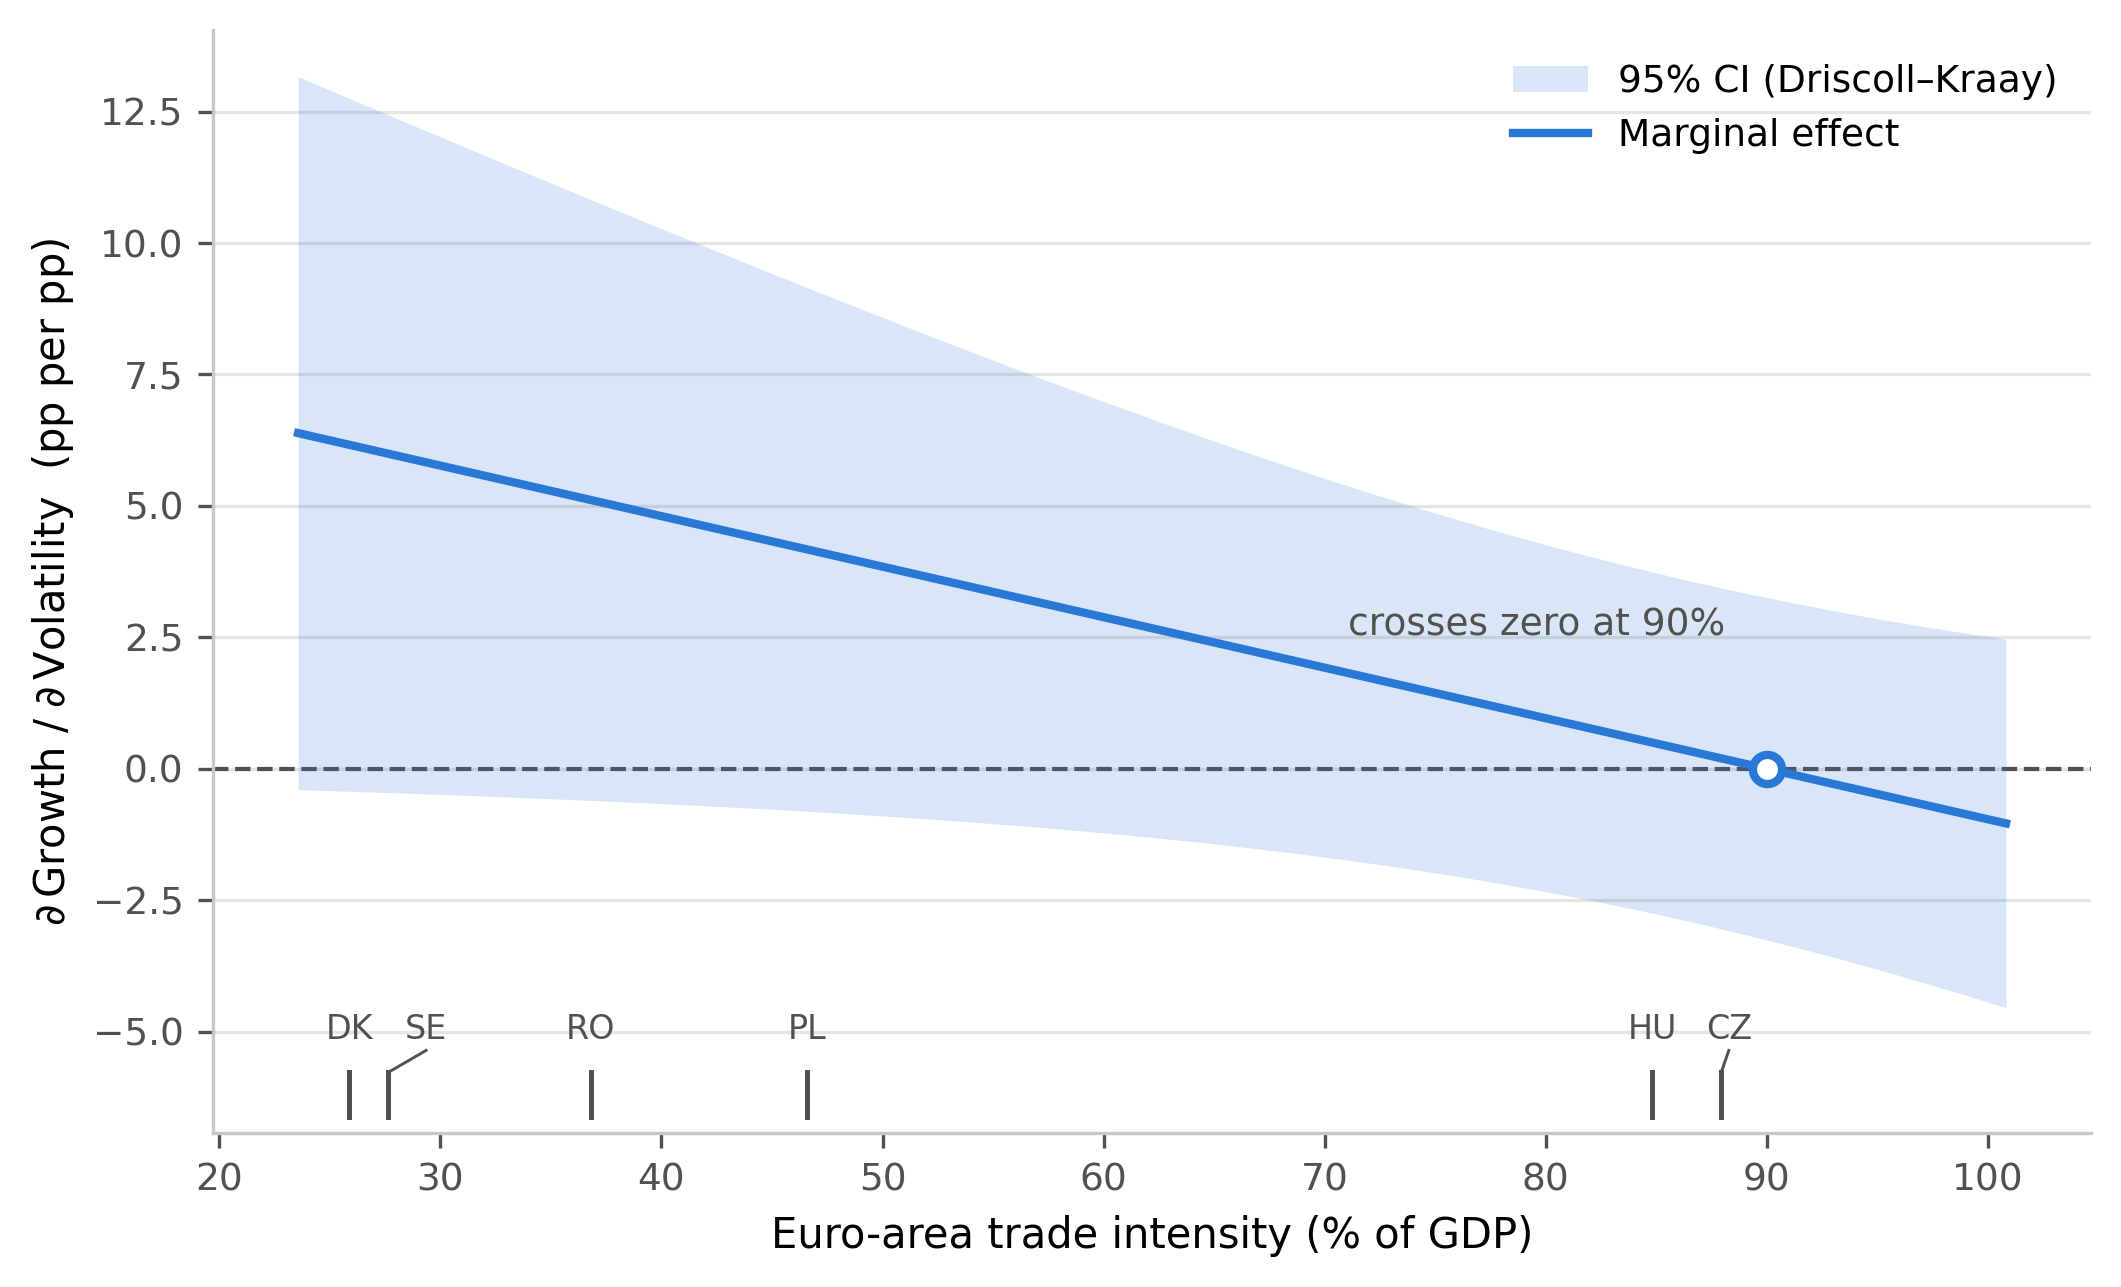
\includegraphics[width=0.75\textwidth]{fig/marginal_effect.png}
    \caption{Marginal effect of volatility on growth by euro area trade intensity with 95\% confidence intervals}
\end{figure}

The joint tests we discussed shows that trade exposure matters but no explanation.
Because the model contain an interaction.
The effect of volatility is not a single number which it changes with a country's trade exposure to the euro area.
This figure \ref{fig:marg_eff} presents the marginal effect of volatility on growth where the line slopes downward across the whole range.
Denmark and Sweden at the left end at around 26 percentage of GDP.
The estimated effect of volatility on growth is positive around 6.3 points.
It fails to 1.1 points by the time trade intensity is near 79 percentage and crosses zero at 90 percentage.
Hungary and the Czech Republic at 85 and 88 percentage respectively.
The shape is expected where a country trade little with the euro area and a moving currency mostly absorbs shocks and the relationship with growth is positive.
The trade increases when the cost volatility imposes on trade grows and offsets the benefit.

\vspace{\baselineskip}

The shaded band includes zero where every point across the range.
The confidence interval covers both positive and negative values.
The lowest p value at 0.066 (See Appendix \ref{appendD} for further details).
This means the negative slope cannot be separated from a flat line at zero.
The pattern matches what the theory predicts.

\vspace{\baselineskip}

It is wider for band at both ends.
The 25 percentage trade intensity runs from -1 to +13 and -4.5 to +2.5 at 100 percentage.
The reason is the marginal effect depends on the interaction coefficient multiplied by the distance from the mean.
The further from the mean the more coefficient's uncertainty carries through.
The largest estimated effects at the ends of the range which is unreliable for the estimates.

\vspace{\baselineskip}
The figure shows no observations in the middle.


\subsection{Diagnostic}\label{subsec:diagnostic}
Jarque-Bera      stat=  53.78  p=0.0000   skew=-0.491  excess kurtosis=+3.129
   H0: normal residuals. Rejection does NOT threaten consistency or unbiasedness
   of the slopes -- only the exact small-sample t and F distributions, which the
   Driscoll-Kraay standard errors replace anyway. Expected with macro data.

\vspace{\baselineskip}

Breusch-Pagan    stat=  39.15  p=0.1224
   H0: constant error variance. Rejection would mean OLS standard errors are
   wrong; the robust estimators already handle it.

\vspace{\baselineskip}

Ramsey RESET 2   F=  0.004  p=0.9479
Ramsey RESET 3   F=  0.722  p=0.4887
   H0: no omitted non-linearity. This is the one test where NON-rejection is the
   good outcome rejection would say the functional form itself is wrong.

\vspace{\baselineskip}

Within-country AR(1)   rho=+0.1446  p=0.1177  n=114
   H0: no first-order serial correlation in the residuals. Significant rho would
   mean the Driscoll-Kraay lag truncation (maxlags=2) is too short.
   Verdict: no evidence of serial correlation.



\subsection{Robustness}\label{sec:robustness}

\begin{table}[H]
    \centering
    \begin{tabular}{lcccc}
        \toprule
        \textbf{Variable} & \textbf{sd\_between} & \textbf{sd\_within} & \textbf{ratio} \\
        \midrule
        vol\_c & 0.179 & 0.140 & 1.278 \\
        trade\_c & 27.941 & 5.466 & 5.112 \\
        vol\_x\_trade & 4.309 & 3.582 & 1.203 \\
        gfcf\_pct\_gdp & 2.692 & 2.319 & 1.161 \\
        hicp & 1.275 & 3.172 & 0.402 \\
        gov\_exp\_pct\_gdp & 5.617 & 2.324 & 2.417 \\
    \end{tabular}
    \caption{Cross-sectional Variation}
    \label{tab:var}
\end{table}

\begin{table}[H]
    \centering
    \begin{tabular}{lccc}
        \toprule
        \textbf{Variable} & \textbf{GARCH} & \textbf{TGARCH} & \textbf{GARCH,No GFCF}\\
        \midrule
        Volatility & +3.691 (p = 0.117) & +3.657 (p = 0.115) & $+5.6159$(p = 0.038)\\
        Trade intensity & +0.051 (p = 0.071) & +0.052 (p = 0.066) & $+0.0227$ (p=0.516)\\
        Volatility × trade & $-0.096$ (p = 0.046) & $-0.093$ (p = 0.051) & $-0.1384$(p=0.029)\\

    \end{tabular}
    \caption{Two-way fixed effects, Driscoll–Kraay standard errors, N = 120. Regression coefficients (standard errors omitted).}
    \label{tab:two_way}
\end{table}

\begin{sidewaystable}
    \centering
    \sisetup{table-number-alignment=center}
    \begin{tabular}{l
                    S[table-format=3.0]
                    S[table-format=-1.4] S[table-format=1.4]
                    S[table-format=-1.4] S[table-format=1.4]
                    S[table-format=-1.4] S[table-format=1.4]
                    S[table-format=2.4]  S[table-format=1.4]}
        \toprule
        & & \multicolumn{2}{c}{Volatility}
          & \multicolumn{2}{c}{Trade intensity}
          & \multicolumn{2}{c}{Volatility $\times$ trade}
          & \multicolumn{2}{c}{Joint test} \\
        \cmidrule(lr){3-4} \cmidrule(lr){5-6} \cmidrule(lr){7-8} \cmidrule(lr){9-10}
        \textbf{Sample} & {\textbf{N}}
        & {Coef.} & {$p$} & {Coef.} & {$p$} & {Coef.} & {$p$} & {$F$} & {$p$} \\
        \midrule
        Full sample                & 120 &  3.6911 & 0.1168 &  0.0510 & 0.0709 & -0.0961 & 0.0462 &  4.7214 & 0.0113 \\
        Excl. DKK (pegged)         & 100 &  3.6796 & 0.2702 &  0.0519 & 0.0149 & -0.0961 & 0.0818 & 13.7952 & 0.0000 \\
        Excl. crisis (2008--09, 2020) & 102 & -0.3114 & 0.8361 &  0.0528 & 0.1512 &  0.0016 & 0.9713 &  1.0778 & 0.3456 \\
        2010--2024 only            &  90 & -2.2944 & 0.2290 &  0.1045 & 0.0011 &  0.0101 & 0.8484 &  5.8781 & 0.0045 \\
        Excl. COVID (2020--21)     & 108 &  4.3601 & 0.0561 &  0.0662 & 0.0268 & -0.0940 & 0.0443 &  5.3945 & 0.0064 \\
        \midrule
        \multicolumn{10}{l}{\emph{Leave-one-country-out}} \\
        \quad Drop CZ              & 100 &  5.3779 & 0.0163 &  0.0931 & 0.0015 & -0.1417 & 0.0040 & 10.1541 & 0.0001 \\
        \quad Drop DK              & 100 &  3.6796 & 0.2702 &  0.0519 & 0.0149 & -0.0961 & 0.0818 & 13.7952 & 0.0000 \\
        \quad Drop HU              & 100 &  3.9802 & 0.1442 & -0.0170 & 0.6048 & -0.1355 & 0.0105 &  3.9792 & 0.0231 \\
        \quad Drop PL              & 100 &  2.8943 & 0.1686 &  0.0295 & 0.3591 & -0.0691 & 0.2076 &  1.9993 & 0.1431 \\
        \quad Drop RO              & 100 &  1.0950 & 0.6699 &  0.0731 & 0.0714 & -0.0673 & 0.1703 &  2.1701 & 0.1218 \\
        \quad Drop SE              & 100 &  4.4230 & 0.0676 &  0.0480 & 0.1780 & -0.1043 & 0.0339 &  3.4291 & 0.0380 \\
        \bottomrule
    \end{tabular}
    \caption{Robustness checks. Two-way fixed effects re-estimated on subsamples,
    Driscoll--Kraay standard errors. Coefficients are reported for centred volatility,
    centred trade intensity and their interaction; centring is held at the full-sample
    origin so the main effects stay comparable across rows. The joint test is a Wald
    $F$ test of $\beta_{\text{trade}} = \beta_{\text{vol} \times \text{trade}} = 0$
    under the Driscoll--Kraay covariance. Since Denmark is the pegged currency, the
    rows \emph{Excl.\ DKK} and \emph{Drop DK} are the same subsample.}
    \label{tab:robust}
\end{sidewaystable}

% The rotated table is a float and cannot be pinned with [H]. Without this barrier
% it drifts past the end of the section and the conclusion is typeset ahead of it.
\FloatBarrier

\section{Limitations}\label{limitation}

The findings above are qualified by several of limitations.
Some concerns what estimates can be taken to mean and others follow from the size of the sample.
Exchange rate volatility and economic growth are jointly determined.
A currency may become volatile because the economy is weakening or just as a volatile currency may weaken the economy.
This design cannot tell which is happening.
A negative coefficient is consistent.
Janus and Riera-Crichton (\citeyear{thorsten_pdf_2015}) address with this finding a variable that moves exchange rate volatility but has no direct effect on growth.
Their case using volatility of a country's commodity terms of trade and isolate the part of volatility that cannot be caused by growth.
There are no similar variables in this analysis.
The estimates in this thesis are association instead of the causal effects.
The volatility is estimated and not observed.
Volatility is not measured directly but estimated in a separate step.
The uncertainty in that estimate is not passed on to the panel regression.
The regression treats the annual volatility average as they were observed data when each carries its own estimation error.
The result is significance overstated by an unknown margin.
Bootstrapping the two steps together would address this.
But it is not performed here.

\vspace{\baselineskip}

The sample is small in both dimensions.
Six countries and twenty years is not much data to work with and it affects the standard errors.
Driscoll-Kraay standard errors reply on having many time periods instead of many countries.
Twenty years is at the low end of what the method needs.
The estimator is consistent and it converges as the sample grows but whether well at this length of panel is a different question.
So the p values presented should be read as approximate instead of exact values.

\vspace{\baselineskip}

The sample cannot support strong claims about stability.
With six countries removing one country means removed a sixth of the observations.
And result will be sensitive to which countries are included.
The crisis years are similar because they are the only period which volatility differs heavily across the sample.
Both problems cannot be fix within this design.
The six countries at two ends of the range with nothing between two groups.
Any estimate of how the effect changes across the range is on the linear form assumed by the specification instead of an observed variation.
The model cannot detect the problem in the relationship where it has no observations.
This follow from which currencies kept their own currencies and was not the study could arranged differently.

\vspace{\baselineskip}

There is limitation on how the variables are measured.
The volatility is measured in nominal terms.
Exchange rates against the euro are used as published without adjusting for relative price levels.
This suits the mechanism the thesis examines since a firm contracting in euro faces the nominal rate but it means the measure cannot separate currency movement from price stability.
A country with unstable inflation will show high nominal volatility.
And the coefficient cannot tell the two apart.
The correlation between volatility and inflation in this sample at 0.29 so the problem present.
A real effective rate would avoid it but it is measuring the movement against the world instead of the euro.
Also GARCH cannot tell a pegged currency.
The model works by describing how volatility changes over time which requires volatility that can changes.
A central bank holds currency close to fixed rate so there is nothing for the model to describe.
This applies to Denmark in the whole sample period in weaker form.
Also Romania under its managed float and Czech Republic exchange rate floor regime during 2013 to 2017.
The estimates still capture how much each currency moved but for three of the six countries they do not describe a volatility process.

 
\thesischapter{Conclusions}
\label{sec:conclusion}

The relationship between exchange rate volatility and economic growth remains unsettled and also the question of how volatility should be measured to find its relationship with growth.
This study add a case instead of an answer.
Exchange rate volatility against the euro shows no independent relationship with growth in the six European Union members that kept their own currencies.
Where a relationship appears it runs trade exposure to the euro area and only in the years of financial crisis.

\vspace{\baselineskip}

Exchange rate volatility does not enter the model independently.
In the country and years fixed effects specification the volatility and its interaction with trade intensity are jointly significant.
There is no evidence that volatility affects growth at an average level of euro area trade exposure.
So the trade exposure is important. 
The joint test of trade intensity and the interaction rejects and the interaction coefficient is negative.
The marginal effect of volatility decreases steadily across the range of trade exposure from positive where trade with the euro are is small share of GDP to negative where it approaches the whole part.
This is the direction of the theory predicts where a country trade little with the euro area a moving currency absorbs shocks.
When it trades increase the cost that volatility imposes on trade cancels that benefit out.
None of these estimates is statistically significant and the confidence interval covers zero at every point.
Our analysis result holds only during financial crisis.
Excluding the crisis years removes the significance.
Excluding the COVID years leaves the estimate unchanged.
The analysis shows it is specific to 2008 to 2009 instead of periods of financial stress in general.

\vspace{\baselineskip}

These findings is different from Morina et al. (\citeyear{morina_effect_2020}) who present a significant negative effect of volatility on growth in a panel of fourteen Central and Eastern European countries.
There are three differences in design can be the reason.
The composition of the sample might be one of the reasons.
Their period covers years in which several members adopted the euro and they present that adoption was itself negative for growth.
Restricting the sample to countries that retained their currencies remove the source of variation.

\vspace{\baselineskip}

Also the measurement of volatility is different.
A real effective exchange rate shows movement against a country's trading partners.
And a euro exchange rate shows movement against the euro and nothing else.
These two do not behave the same and particularly for economics whose trade is diversified beyond the euro area.
The third difference is the model and it is the most important one.
Estimated only with country fixed effect finds a negative and significant coefficient on volatility.
This result changed after adding year affects which absorb what happened to all six countries in 2009 and would read as an effect of volatility.
It is not possible to say here which of the three is important.
The estimate is sensitive to the treatment of common shocks deserves attention.
The trade mechanism was also the least conclusive of the three from Morina et al. (\citeyear{morina_effect_2020}) study.
In both studies the interaction between volatility and trade exposure is harder to identify the direct effects.

\vspace{\baselineskip}

In general there are three directions can be address for further research.
The instrument for exchange rate volatility and following Janus and Riera-Crichton (\citeyear{thorsten_pdf_2015}) who use volatility of commodity terms of trade.
And a larger panel that extending to European countries outside the Union would fill the gap in the trade intensity range and reduce the sensitivity of the estimate to individual countries.
And estimating the volatility model and the panel regression together by bootstrap would produce standard errors that reflect the uncertainty in the first step which this analysis does not account for.


 
\thesischapter{Bibliography}\label{sec:bibliography}
\nocite{*}
\printbibliography[heading=none, keyword=paper]
 
\thesissection{List of Appendices}\label{sec:appendix_list}
\subsection{Appendix A}\label{appendA}

\begin{table}[H]
    \centering
    \caption{Correlation matrix}
    \vspace{\baselineskip}
    \begin{tabular}{lrrrrrr}
        \toprule
        & (1) & (2) & (3) & (4) & (5)&(6) \\
        \midrule
        $growth$(1)& 1.00 & -0.08 & 0.04 & 0.12 & -0.02 & -0.36 \\
        $vol$ (2) & -0.08 & 1.00 & 0.29 & 0.09 & 0.29 & -0.00 \\
        $trade$ (3)& 0.04 & 0.29 & 1.00 & 0.24 & 0.21 & -0.22 \\
        $gfcf$ (4)& 0.12 & 0.09 & 0.24 & 1.00 & 0.26 & -0.36 \\
        $hicp$ (5)& -0.02 & 0.29 & 0.21 & 0.26 & 1.00 & -0.16 \\
        $govexp$ (6)& -0.36 & -0.00 & -0.22 & -0.36 & -0.16 & 1.00 \\
        \bottomrule
    \end{tabular}
    \vspace{\baselineskip}
    \caption*{\footnotesize Source: Own study.}
\end{table}

\subsection{Appendix B}\label{appendB}
\begin{table}[H]
    \centering
    \caption{GARCH(1,1)-t estimates.}
    \vspace{\baselineskip}
    \begin{tabular}{lcccc}
        \toprule
        \textbf{Currency} & \textbf{$\omega$} & \textbf{$\alpha+\beta$} & \textbf{$\nu$} & \textbf{Note} \\
        \midrule
        CZK & 0.00011 & 0.999994 & 5.09 & $\omega$ at floor; managed regime \\
        DKK & 0.000004 & 0.999994 & 3.86 & ERM II band \\
        HUF & 0.00155 & 0.996745 & 7.78 &  \\
        PLN & 0.00136 & 0.998716 & 6.53 &  \\
        RON & 0.00010 & 0.999994 & 4.24 & $\omega$ at floor; managed regime \\
        SEK & 0.00204 & 0.988569 & 7.82 &  \\
        \bottomrule
    \end{tabular}
    \vspace{\baselineskip}
    \caption*{\footnotesize Source: Own study. }
    \label{app:garch}
\end{table}

\subsection{Appendix C}\label{appendC}

\begin{table}[H]
    \centering
    \caption{P-values under alternative covariance estimators.}
    \vspace{\baselineskip}
    \begin{tabular}{llrrr}
        \toprule
        \textbf{Spec.} & \textbf{Variable} & \textbf{p (OLS)} & \textbf{p (HAC)} & \textbf{p (clu)} \\
        \midrule
        Model 1 & $vol$                & 0.311 & 0.333 & 0.246 \\
         & $trade$           & 0.982 & 0.983 & 0.987 \\
         & $vol x trade$  & 0.199 & 0.223 & 0.039 \\
         & $gfcf$                      & 0.939 & 0.948 & 0.950 \\
         & $hicp$                      & 0.886 & 0.867 & 0.766 \\
         & $govexp$    & 0.003 & 0.001 & 0.004 \\
        \midrule
        Model 2 & $vol$                & 0.046 & 0.027 & 0.045 \\
         & $trade$          & 0.219 & 0.255 & 0.134 \\
         & $Vol x trade$ & 0.522  & 0.440 & 0.450 \\
         & $gfcf$                      & 0.004 & 0.011 & 0.001 \\
         & $hicp$                      & 0.625 & 0.609 & 0.511 \\
         & $govexp$    & 0.001 & 0.002 & 0.025 \\
        \midrule
        Model 3 & $vol$                & 0.064 & 0.081 & 0.198 \\
         & $trade$           & 0.233 & 0.115 & 0.307 \\
         & $Vol x trade$ & 0.058  & 0.023 & 0.042 \\
         & $gfcf$                      & 0.007 & 0.001 & 0.030 \\
         & $hicp$                      & 0.120 & 0.085 & 0.218 \\
         & $govexp$    & 0.832 & 0.806 & 0.871 \\
        \bottomrule
    \end{tabular}
    \vspace{\baselineskip}
    \caption*{\footnotesize Source: Own study. Note: OLS = ordinary least squares; HAC = Newey-West; clu = clustered by country.}
    \label{tab:se_alt}
\end{table}

\subsection{Appendix D}\label{appendD}

\begin{table}[H]
    \centering
    \vspace{\baselineskip}
    \caption{Marginal effect of volatility on growth}
    \begin{tabular}{lcccc}
        \toprule
        \textbf{Quantile} & \textbf{Trade intensity} &
        $\partial\mathit{Growth}/\partial\mathit{Vol}$ & \textbf{SE} & \textbf{p} \\
        \midrule
        5th   & 24.96 & $6.251$   & 3.354 & 0.066 \\
        25th  & 28.28 & $5.932$   & 3.217 & 0.069 \\
        50th  & 40.47 & $4.761$   & 2.734 & 0.085 \\
        75th  & 78.54 & $1.103$   & 1.675 & 0.512 \\
        95th  & 95.64 & $-0.540$  & 1.686 & 0.749 \\
        \bottomrule
    \end{tabular}
    \vspace{\baselineskip}
    \caption*{\footnotesize Source: Own study.}
    \label{tab:mar_eff_vol}
\end{table}
 
\end{document}